\chapter{A Python Package for SMBO} \label{ch:code}


In exploring this topic, I have built a Python package for performing sequential model-based optimization, simply named \texttt{smbo}. My goal in making it was to construct well-made code, that will be immediately useful as a pedagogical tool (indeed, it was used to generate several figures in this thesis \ref{}), open source and available online, and documented and designed such that further development of the code base is easy; perhaps some day \texttt{smbo} will evolve into a cutting-edge free optimization package, used to optimize all sorts of blackbox functions all over the globe, maintained by an international team of elite open-source hackers. Though at present the package only implements the EGO algorithm, its modular, hybrid object-oriented/functional construction allows for further SMBO processes to be defined and implemented easily. \texttt{smbo} is available on the Python Package Index, and can be downloaded and installed with a single command on any computer with Python 2.7.9 or later.\footnote{\texttt{sudo pip install smbo}}

As a good portion of the work in this thesis went into software design and engineering (subjects not taught at Reed College), I will here present the code behind the \texttt{smbo} package on the highest level. This discussion will inform the reader's mathematical understanding of SMBO processes, covering design decisions, identifying runtime bottlenecks, and the crucial components upon which the performance of any SMBO implementation rely. This chapter will also serve as an introduction to the official documentation of the \texttt{smbo} package, which is included as an appendix to this thesis.

\section{Design}\ref{sec:design}

The three-stage SMBO cycle, illustrated earlier in Figure \ref{fig:smbo_cycle}, presents a clear opportunity for a modular implementation of sequential model-based optimizers. It can be conceived of mathematically as three functional components: an objective function $F$, a model-producing function $M$, and a sample-point-selecting function $S$. Where $X$ denotes a point in $F$'s input space, and $\mathbf{X},\mathbf{Y}$ represent vectors of $X$s and their corresponding $F(X)$s, the three stages can expressed functionally as,

\begin{enumerate}
\item $F(\mathbf{X})=\mathbf{Y}$
\item $M(\mathbf{X},\mathbf{Y}) = (\hat{y},\hat{err}_{\hat{y}})$
\item $S(\hat{y},\hat{err}_{\hat{y}}) = x_{new}$.
\end{enumerate}


The technical goal of the \texttt{smbo} package is to provide a class, called \texttt{smb$\_$optimizer}, which generically handles and passes arguments between the above three functions to perform the iterative SMBO process. Since this thesis is largely concerned with the case where $S$ is defined by expected improvement maximization (Section \ref{sec:exp_imp}), this stage of the process is implemented by a fixed class method of \texttt{smb$\_$optimizer}. The other two functions, $F$ and $M$, are callables passed upon initialization to the \texttt{smb$\_$optimizer} class. This information is summarized on the familiar SMBO loop in Figure \ref{fig:smbo_loop_II}, and the technical details of the \texttt{smb$\_$optimizer} class's initialization are described in Figure \ref{fig:smb_optimizer} .

\begin{figure}[h]
	\centering
	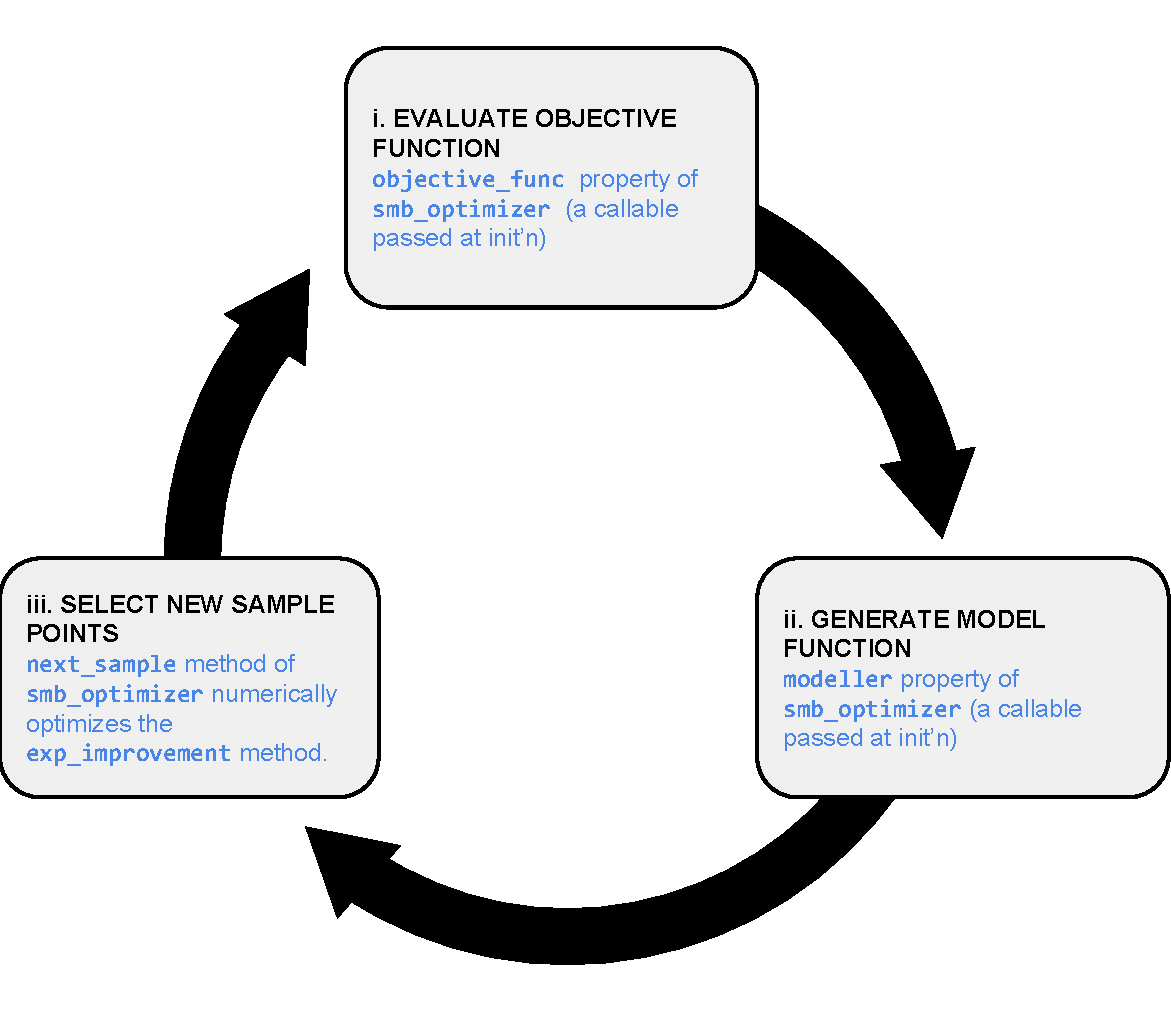
\includegraphics[width=0.75\textwidth]{smbo_loop_II}
	\caption{An instantiation of an SMBO process consists of a single \texttt{smb$\_$optimizer} object. Here the SMBO loop is labeled with the type of its implementation in the \texttt{smb$\_$optimizer} class.}
	\label{fig:smbo_loop_II}

\end{figure}


The EGO algorithm, our prototypical SMBO process, is defined by a particular choice of modeller $M$, i.e., the DACE model. This is accomplished by the module \texttt{dace}, which is the primary component of \texttt{smbo} meriting the description ``functional/object-oriented hybrid'' mentioned in the introduction to this chapter. \texttt{dace} contains two pieces: a class \texttt{dace$\_$model} which has various methods to implement the calculations defined and derived in Chapter \ref{ch:ego}, including the formulation of $\hat{y}$ and $\hat{err}_{\hat{Y}}$; and a functional wrapper $dace_func$ which behaves exactly as the ideal functional modeller $M(\mathbf{X},\mathbf{Y}) = (\hat{y},\hat{err}_{\hat{y}})$. That is to say, \texttt{dace$\_$func} takes as input two vectors $(\mathbf{X},\mathbf{Y})$, uses them to initialize an instance of the \texttt{dace$\_$model} class, then retrieves $\hat{y}$ and $\hat{err}_{\hat{Y}}$ using methods of that \texttt{dace$\_$model}, returning them as output.

There were two factors that influenced the decision to implement the DACE model in this function-wrapped-class kind of way.
First, there is the standard conceptual appeal of functional programming---here, we can appreciate the mathematical purity of a code module that behaves exactly as the generic modelling function $M$ described above, mapping sample points to predictive models. This also makes clear the modular distinction between the central \texttt{smb$\_$optimizer} and its modeller---as far as an \texttt{smb$\_$optimizer} instance is concerned, the modeller is a black box which produces models from sample points. On the other hand, the functional paradigm makes it awkward to allow an \texttt{smbo} package user to experiment with the specifics of a particular modelling function, e.g. to see the results of modifying traditionally internal DACE parameters, such as the characteristic parameter vectors $\mathbf{P}$ and $\mathbf{\theta}$ (the reader should see Section \ref{sec:dace} if they've forgotten why one might want to play with these parameters). 


% The smb_optimizer documentation
\begin{minipage}{\textwidth}
\begin{framed}
\begin{fulllineitems}
\phantomsection\label{index:smbo.smb_optimizer.smb_optimizer}\pysiglinewithargsret{\strong{class }\code{smbo.smb\_optimizer.}\bfcode{smb\_optimizer}}{\emph{domain}, \emph{objective\_func}, \emph{modeller}, \emph{init\_sampler=None}}{}
An object that, given an input domain, objective function, and modelling strategy, implements sequential model-based optimization to search for a global minimum of the objective function.
\begin{quote}\begin{description}
\item[{Initialization Arguments}] \leavevmode\begin{itemize}
\item {} 
\textbf{\texttt{domain}} (\emph{list}) -- a list whose \(i^{th}\) element is the \((lower\ bound,\ upper\ bound)\) pair
describing the domain of interest in the \(i^{th}\) input dimension. The length
of this list defines the dimension of input space, denoted \(k\). This smb\_optimizer
then optimizes the \(k\)-rectangle defined by the domain arg.

\item {} 
\textbf{\texttt{objective\_func}} (\emph{function}) -- a function (or any object with a suitable \_\_apply\_\_ method)
that maps \(k\)-vectors to floats. The goal of an smb\_optimizer is to minimize this
function over the domain defined above.

\item {} 
\textbf{\texttt{modeller}} (\emph{function}) -- a function (or any object with a suitable \_\_apply\_\_ method) that maps a
tuple \((X,Y)\), which describes the input and known output values for a list of sample points to a tuple of functions
\((\hat{y},\ \hat{\sigma}^2)\).
\(\hat{y}\) represents the model's best estimate of \code{objective\_func(X)}, and \(\hat{\sigma}^2\)
is the estimated error of that prediction.

\item {} 
\textbf{\texttt{init\_sampler}} (\emph{function}) -- a function which will select initial sample points, informing the zero-generation model.
If left unspecified, is by default set to a \(2k+2\)-sample latin hypercube over the domain,
created with \code{smbo.latin\_hypercube}.

\end{itemize}


\item[{Attributes---Set at Initialization}] \leavevmode\begin{itemize}

\item{}
\textbf{\texttt{X}} (\emph{list}) -- The list of points where \code{objective\_func} has been evaluated already

\item {} 
\textbf{\texttt{Y}} (\emph{list}) -- The list of associated objective function values.

\item {} 
\textbf{\texttt{pred\_y}} (\emph{function}), \textbf{\texttt{pred\_err}} (\emph{function}) -- The predictor and predicted error surfaces; the output of \code{modeller(X,Y)}.

\item {} 
\textbf{\texttt{f\_min}} (\emph{dict:}\texttt{\{x:\_,y:\_\}}) -- The sample point that is the current known minimum.


\end{itemize}


\end{description}\end{quote}

% expected improvement
\index{exp\_improvement() (smbo.smb\_optimizer.smb\_optimizer method)}

\begin{fulllineitems}
\phantomsection\label{index:smbo.smb_optimizer.smb_optimizer.exp_improvement}\pysiglinewithargsret{\bfcode{exp\_improvement}}{\emph{x\_new}}{}Calculates the expected improvement at \code{x\_new}, by estimating from \code{pred\_y} and \code{pred\_err} the probability that an evaluation of \code{objective\_func} at \code{x\_new} would find a value lower than \code{f\_min}.


\end{fulllineitems}


% sample
\begin{fulllineitems}
\phantomsection\label{index:smbo.smb_optimizer.smb_optimizer.sample}\pysiglinewithargsret{\bfcode{sample}}{}{}
Chooses the next sample point by maximizing \code{exp\_improvement}.
Evaluates \code{objective\_func} there, updating \code{X} and \code{Y}. Updates \code{pred\_y} and \code{pred\_err} to the output of \code{modeller(X,Y)}.
\end{fulllineitems}


% take_samples
\index{take\_samples() (smbo.smb\_optimizer.smb\_optimizer method)}
\begin{fulllineitems}
\phantomsection\label{index:smbo.smb_optimizer.smb_optimizer.take_samples}\pysiglinewithargsret{\bfcode{take\_samples}}{\emph{stopping\_improvement=0.01}, \emph{max\_iters=100}, \emph{plot\_dims=None}}{}
Completes the SMBO loop until the best expected improvement is below \code{stopping\_improvement}, or \code{max\_iters} times. Optionally, produces plots of the prediction and error surfaces at every iteration.
\end{fulllineitems}






\end{fulllineitems}


\end{framed}

\captionof{figure}{A summary of the documentation of the \texttt{smb$\_$optimizer} class. To find a global minimum, initialize an \texttt{smb\_optimizer}, call \texttt{take\_samples}, then look at \texttt{f\_min}.}\label{fig:smb_optimizer}

\end{minipage}



% The dace documentation
\begin{minipage}{\textwidth}
\begin{framed}
\begin{fulllineitems}
\phantomsection\label{index:smbo.models.dace}\pysiglinewithargsret{\strong{class }\code{smbo.models.}\bfcode{dace}}{\emph{X}, \emph{Y}}{}
A class that implements the DACE model to produce predictor and error surfaces from sample points
\begin{quote}\begin{description}
\item[{Parameters}] \leavevmode\begin{itemize}
\item {} 
\textbf{\texttt{X}} (\emph{list}) -- a list of input vectors

\item {} 
\textbf{\texttt{Y}} (\emph{list}) -- a list of observed objective values

\end{itemize}

\item[{Returns}] \leavevmode
(pred\_y,pred\_err): two functions, each k-to-1, where k is the dimension of the input space, representing the DACE predictor and predicted error at any point in input space.

\item[{Return type}] \leavevmode
tuple

\end{description}\end{quote}
\index{conc\_likelihood() (smbo.models.dace method)}

\begin{fulllineitems}
\phantomsection\label{index:smbo.models.dace.conc_likelihood}\pysiglinewithargsret{\bfcode{conc\_likelihood}}{\emph{new\_P=None}, \emph{new\_Q=None}}{}~\begin{quote}\begin{description}
\item[{Parameters}] \leavevmode\begin{itemize}
\item {} 
\textbf{\texttt{new\_P}} (\emph{list}) -- an \(n\)-vector resetting the \(p\) parameter of the DACE model

\item {} 
\textbf{\texttt{new\_Q}} (\emph{list}) -- an \(n\)-vector resetting the \(q\) or :math:{}`        heta{}` parameter of the DACE model

\end{itemize}

\end{description}\end{quote}

Returns the statistical likelihood of the current DACE parameters \code{P' and :code:{}`Q', given the data :code:{}`X} and \code{Y}.

\end{fulllineitems}
\end{fulllineitems}

\end{framed}

\captionof{figure}{Selected documentation for the \texttt{dace} model class.}\label{fig:dace_doc}

\end{minipage}

\section{Optimization Subroutines}
The EGO algorithm as implemented by \texttt{smbo.smb$\_$optimizer} and \texttt{smbo.dace} together involves two global optimization steps as subroutines: the fitting of the DACE model by maximizing the likelihood of its characteristic parameters (Section \ref{sec:max_lik}), and the SMBO-standard selection of successive sample points by maximizing the expected improvement function. These two steps are the main performance and runtime bottlenecks of the SMBO algorithm, at least as implemented by my \texttt{smbo} package.

I'll discuss why I say they are bottlenecks.

Jones et al were cleverer about their optimizations, but they used DACE-specific reasoning. It is likely that alternative model choices will be ripe for similarly fruitful analysis.

Despite computational costs, it is important to remember (reference ProtoLife) that the blackbox functions being optimized could well be just orders and orders of magnitude harder to compute, e.g., when your blackbox function involves a robot performing 600 chemical experiments.

